\chapter{Methodology}
In this section a performance model for understanding the runtime characteristics of deep learning models is outlined. To understand these characteristics, the underlying factors that affect it need to be understood first. 
\section{Problem Space}
The inference performance of a deep learning model is mainly affected by two major parts, the structure of the model itself and the hardware environment where it gets deployed. A third factor is the serving framework.

\subsection{Deep Learning}
Deep learning models describe neural network with many layers and hidden units, the most popular being convolutional neural networks and recurrent neural networks right now. %This increased amount of layers leads to complex mathematical calculations.
\subsubsection{Convolutional Neural Network}
This special subclass of neural network achieved wide success in the field of object recognition and detection in images. 
\subsubsection{Recurrent Neural Network}
Recurrent neural network are made for the processing of sequences and made a lot a progress in the fields of voice recognition.


\begin{itemize}
    \item parameter von Modellen
    \item Was für Einfluss haben diese Parameter?
\end{itemize}
\subsection{Hardware Evironment}
\begin{itemize}
    \item constraints in hardware
    \item neue accelarators
    
\end{itemize}
\section{Deployment}
Model deployment describes the process of deploying a trained machine learning model to a production environment.
\subsection{Edge Deployment}
\begin{itemize}
    \item Was ist Edge (Beispiele)
    \item Was macht Edge aus?
\end{itemize}
\subsection{Cloud Deployment}
\begin{itemize}
    \item Was ist cloud?
    \item Was macht cloud aus
\end{itemize}
\section{Deployment Trade-offs}
\begin{itemize}
    \item Unterschiede aus verschiedenen deployment optionen
\end{itemize}
Metriken:
\begin{itemize}
    \item Welche Metriken (inference time....)
    \item Wie werden die Metriken gemessen?
    \item Wo werden Metriken gemessen?
\end{itemize}
\begin{figure}[H]
\centering
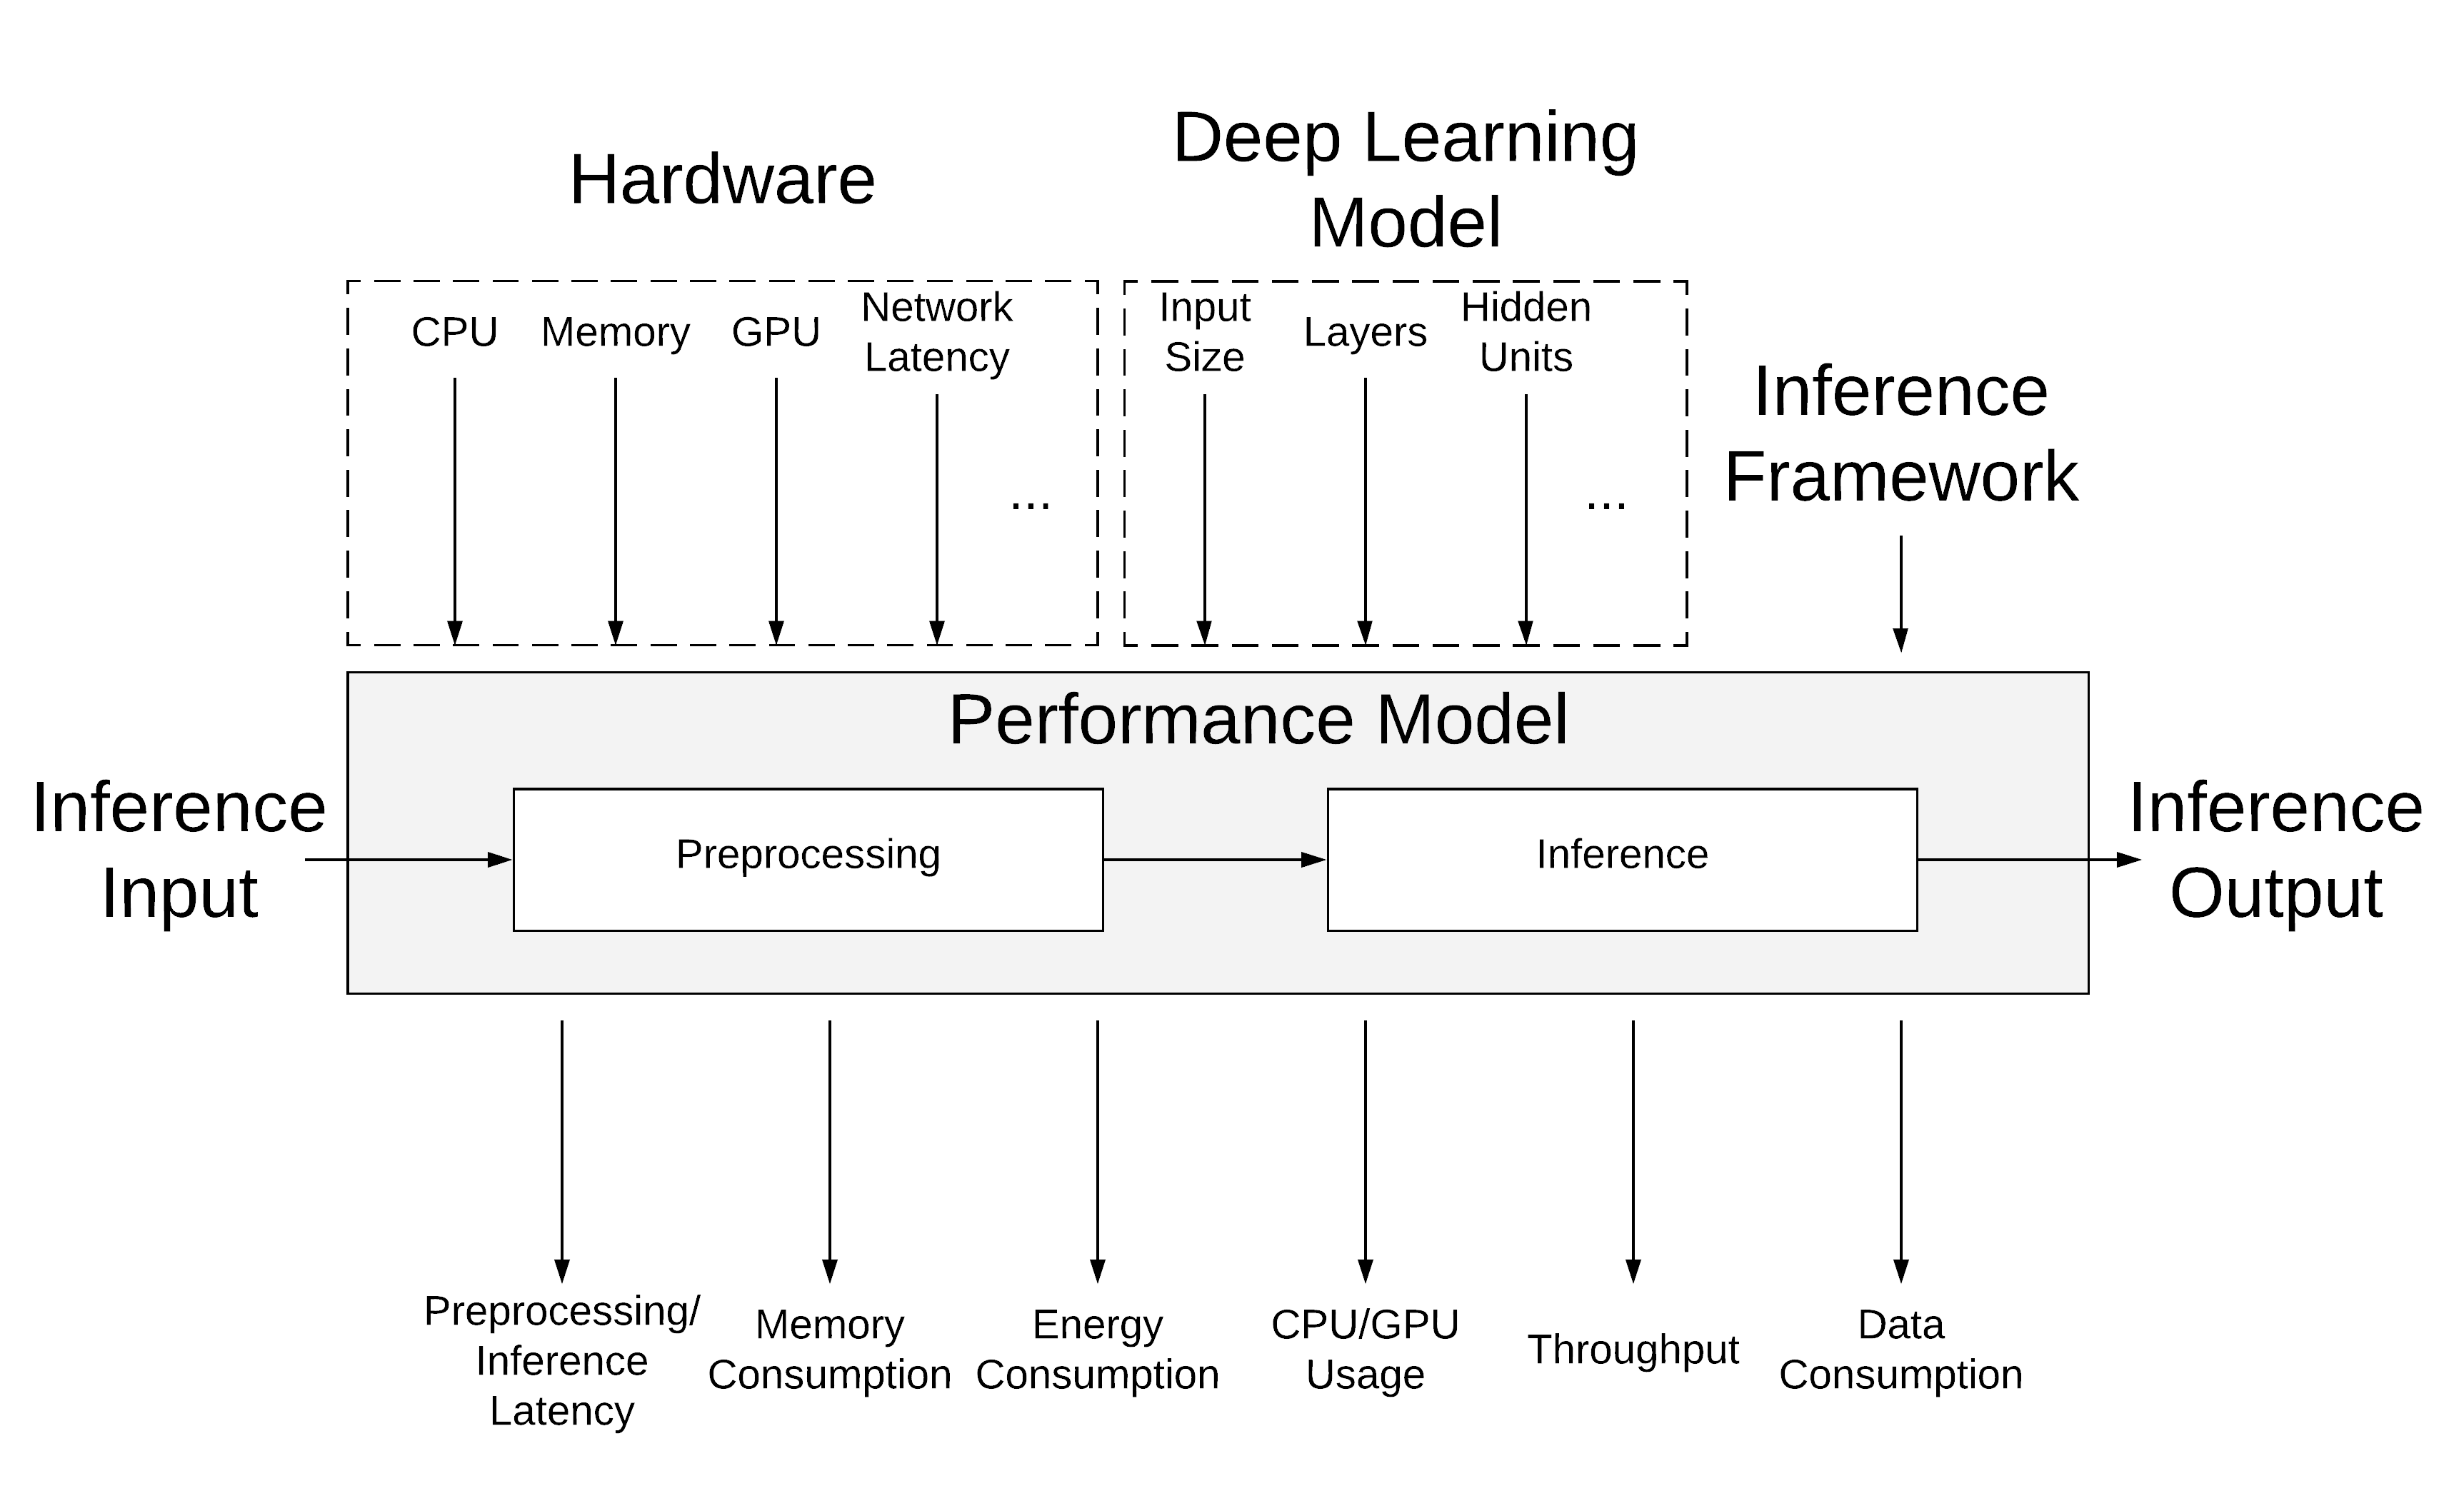
\includegraphics[width=0.9\textwidth]{./Bilder/trade_offs.png}
\caption{Performance Model}
\label{fig:perf_model}
\end{figure}
\endinput 